\documentclass[10pt,twoside,twocolumn,openany]{dndbook}
\let\chaptername\relax

\usepackage[spanish]{babel}
\usepackage[utf8]{inputenc}
\usepackage[singlelinecheck=false]{caption}
\usepackage{lipsum}
\usepackage{listings}
\usepackage{shortvrb}
\usepackage{stfloats}
\usepackage{ifoddpage}
\usepackage{graphicx}
\usepackage{tikz}
\usepackage{hyperref}

\hypersetup{
  colorlinks=true,
  linkcolor=red,
  pdfauthor={Moisés Serrano Samudio},
  pdftitle={El retrato maldito},
  pdfsubject={one-shot},
  pdfkeywords={Dungeon and Dragons, DnD, 5e, exploración}
}

\DndSetFonts[section-style = \linespread{.9} \color{titlered} \LARGE \scshape \RaggedRight]

\title{El retrato maldito\\
\large One shot para personajes de nivel 3}
\author{linkmoises}
\date{\today}

\begin{document}

%% Portada
\newpage
\thispagestyle{empty}
\mbox{}
\begin{figure}
  \begin{tikzpicture}[remember picture,overlay]
    \begin{scope}
    \node [xshift=0cm,yshift=0cm] at (current page.center){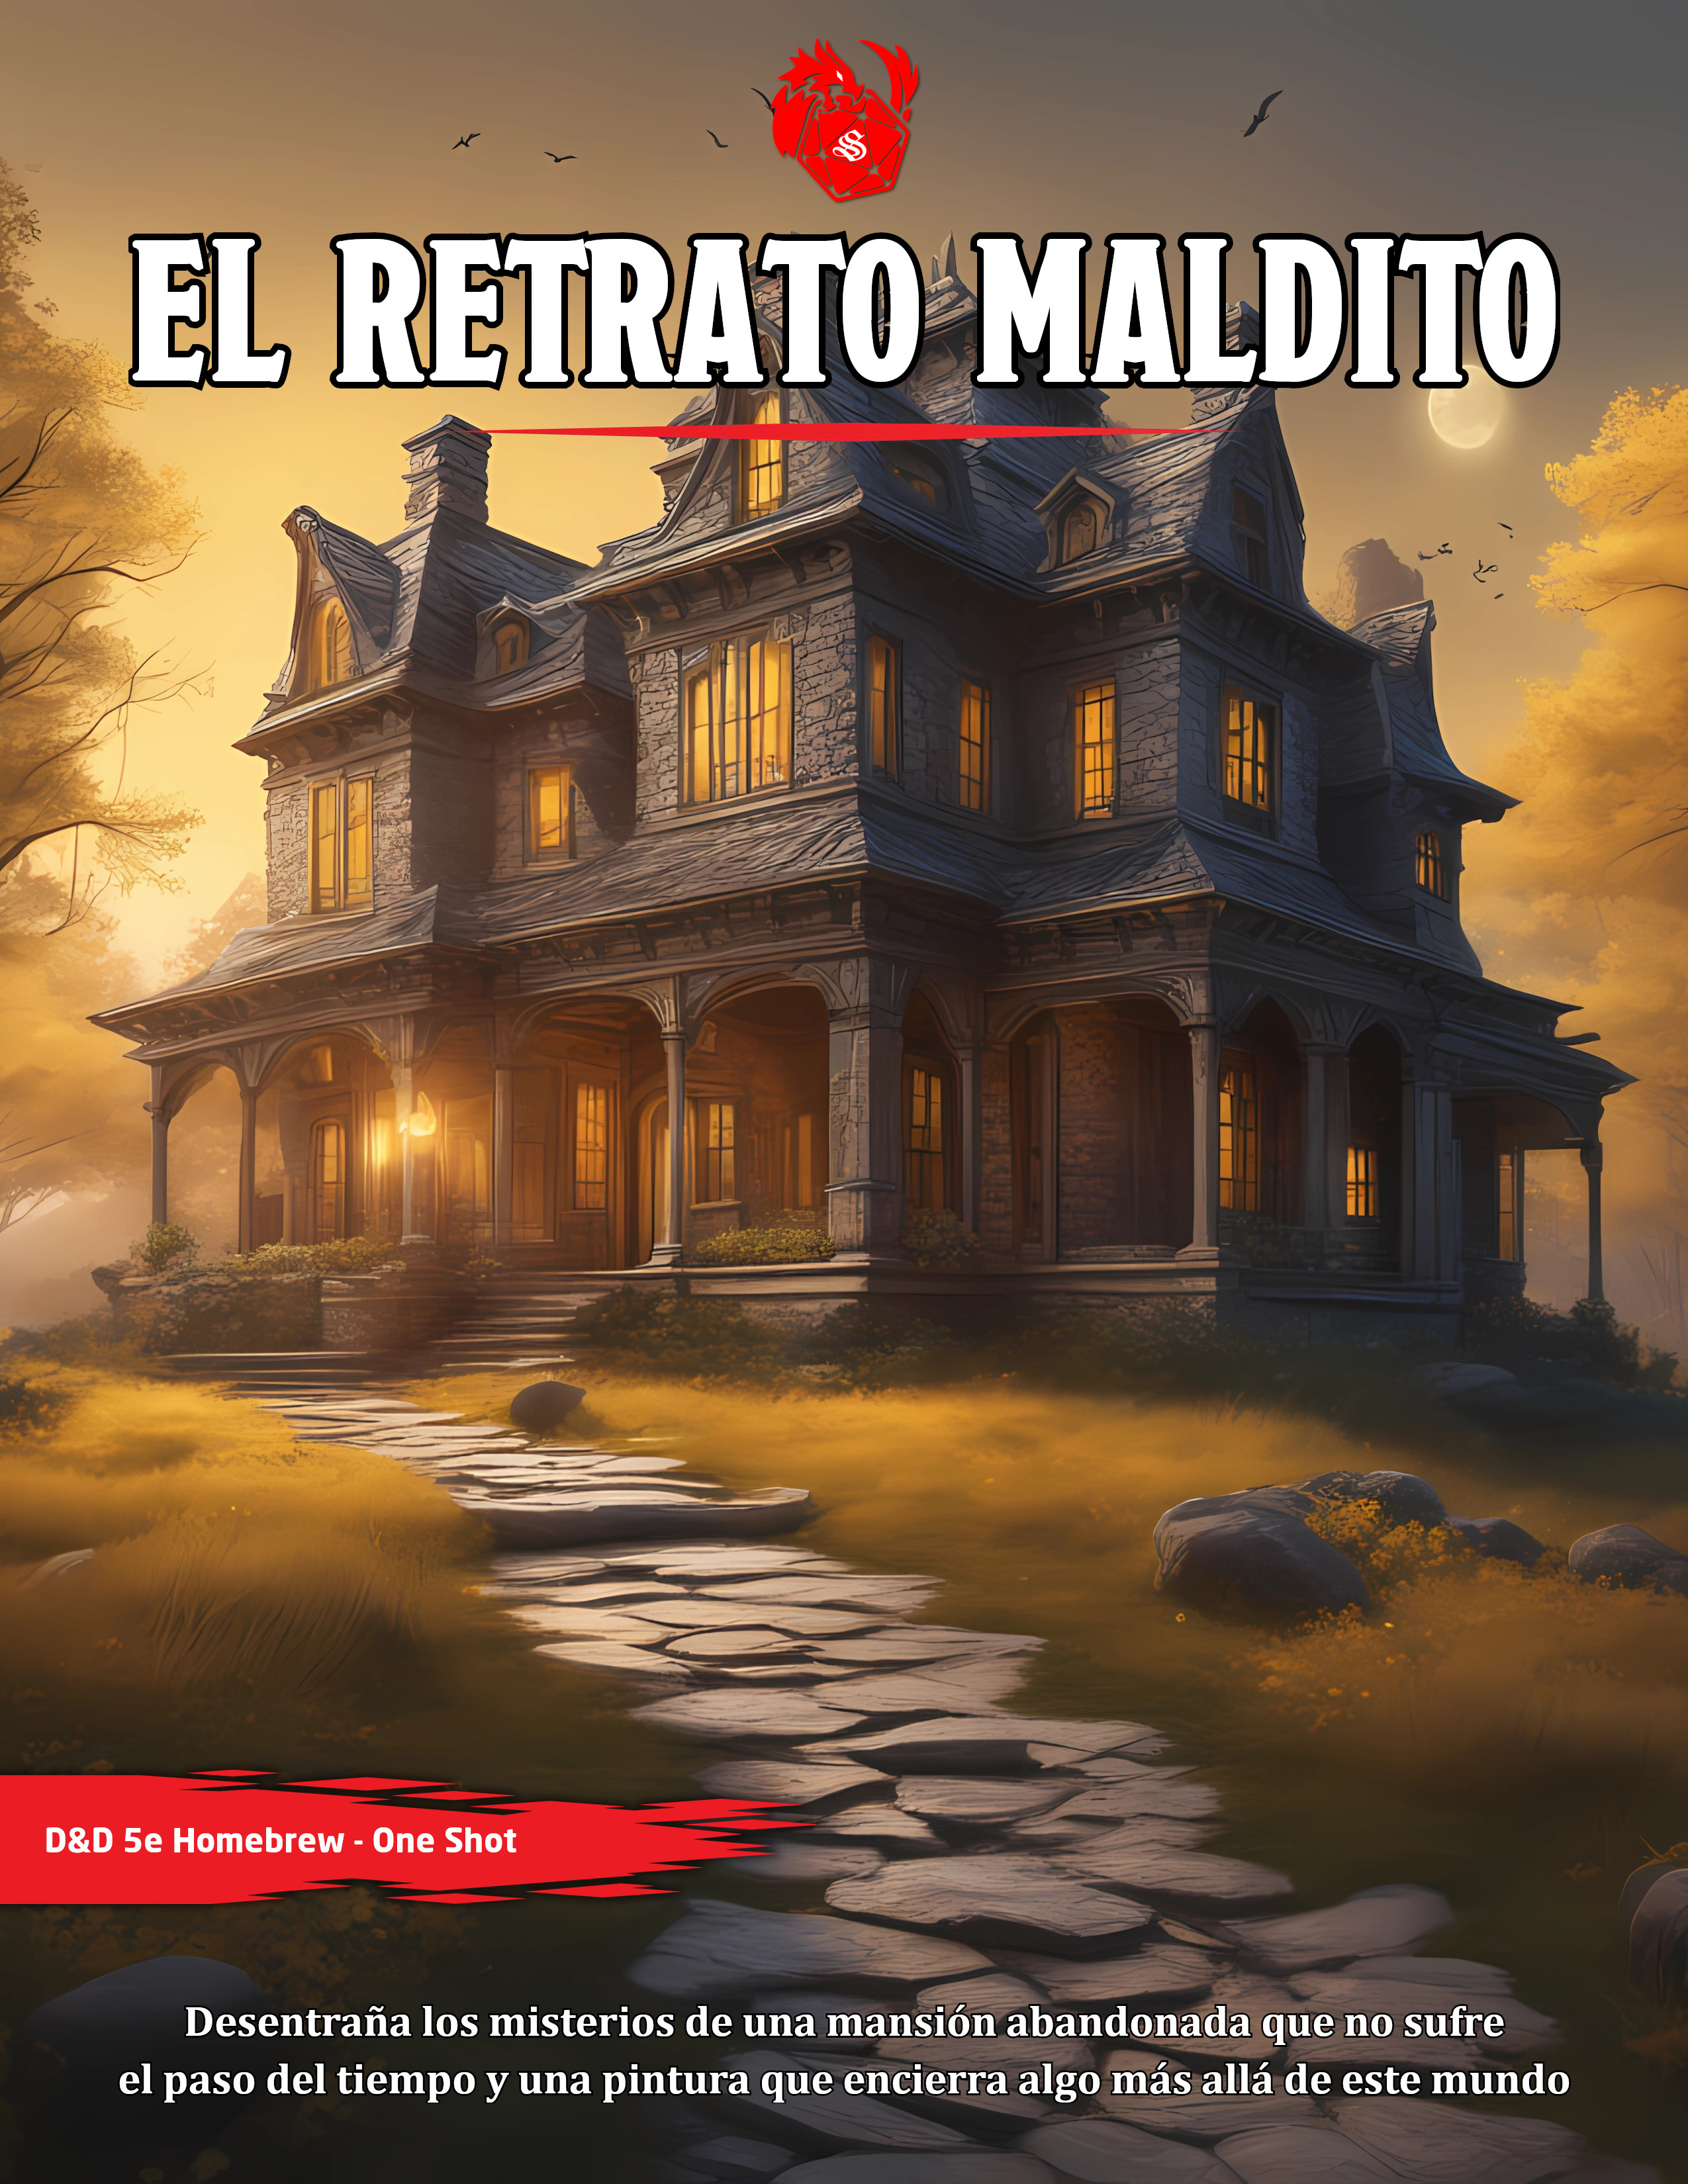
\includegraphics[width=\paperwidth]{covers/3-el-retrato-maldito.jpg}};
    \end{scope}
  \end{tikzpicture}
\end{figure}
%% Finaliza portada

\frontmatter

\maketitle

\mainmatter

\part*{El retrato maldito}

\chapter*{El retrato maldito}
\addcontentsline{toc}{chapter}{El retrato maldito}

\DndDropCapLine{E}{l sol se pone en el horizonte} teñiendo los cielos con tonos de naranja y 
púrpura, mientras te acercas a la ciudad de Neverwinter. La brisa fresca del mar se mezcla con 
el aroma de las flores silvestres que bordean el camino. Neverwinter, una ciudad de renombre en los
Reinos Olvidados, se extiende ante ti con sus calles bulliciosas y su animada vida nocturna.

En el corazón de esta metrópolis vibrante, las luces de las tabernas y los puestos de mercado 
comienzan a brillar, creando un espectáculo de colores y sonidos que invita a aventureros y 
comerciantes por igual. Sin embargo, esta noche, tu atención se centra en un enigma mucho más 
antiguo y oscuro: Villa Argentum.

\begin{DndReadAloud}
Situada en las afueras de Neverwinter, en una zona aislada y rodeada por un denso bosque ancestral,
Villa Argentum se yergue como un testigo silencioso del pasado. La mansión, de dos niveles, un 
ático y un sótano misterioso, se alza imponente y enigmática en medio del paisaje natural. Sus 
muros de piedra gris se erigen como guardianes antiguos, y sus ventanas altas han sido cubiertas
con tablones de madera, parecen ocultar secretos que la ciudad nunca ha conocido.

A medida que te acercas a Villa Argentum, sus torretas y picos de techos puntiagudos se recortan 
contra el cielo crepuscular, creando una imagen digna de un cuento de hadas sombrío. Los jardines 
que rodean la mansión están cubiertos por una maraña de rosales silvestres y setos descuidados, 
otorgándole una belleza marchita y encantadora.
\end{DndReadAloud}

\section{Presentación y gancho de aventura}

Villa Argentum lleva muchos, muchos años abandonada. Sirius Belmont, la última persona que vivió 
allí, se fue de la ciudad hace 100 años, sin que nadie recuerde aparentemente el motivo. Durante 
las últimas décadas, la casa ha permanecido abandonada y ha sido fruto de todo tipo de rumores y 
especulaciones.

Ha habido varios intentos de volverla a habitar, pero todos aquellos que se mudaron allí, acabaron
por marcharse al poco tiempo, argumentando que algo raro pasaba entre sus muros. Con el paso del 
tiempo, la propiedad dejó de provocar interés... hasta ahora.

La leyenda de Villa Argentum habla de un linaje olvidado y un pacto oscuro, y es ahora, en este
atardecer inquietante, que te has encontrado con la oportunidad de descubrir la verdad que se 
esconde tras sus puertas.

Los aventureros son ya héroes que empiezan a tener algo de fama. Dependiendo de la conformación 
del grupo o del tiempo de disponible, diversos ganchos de aventura pueden ser utilizados.

Los personajes reciben un mensaje de un viejo amigo o aliado que dice haber conocido a un 
descendiente de los dueños de Villa Argentum. El mensaje les informa que esta persona esta 
dispuesta a pagar una importante suma de piezas de oro ruega que acudan a la mansión a investigar
y disipar los rumores que se escuchan sobre Villa Argentum.

Otro gancho que puede ser utilizado sería que los personajes se enteran de que Villa Argentum está 
a la venta y se sienten atraídos por la oportunidad de adquirir una propiedad legendaria. Cuando 
llegan, se encuentran con una persona que se presenta como descendiente de los dueños de la 
mansión que se había criado muy lejos de aquel lugar y que recibía la noticia que la heredaba,
pero no esta interesado en vivir en ella por lo que desea venderla, pero también dilucidar los
rumores que existen sobre Villa Argentum.


\section{Sirius: Un descendiente carismático}

\begin{figure}
  \centering
  
\includegraphics[width=0.9\columnwidth]{media/sirius-belmont.png}
  \caption{Lord Sirius Belmont}
\end{figure}

Al llegar a Villa Argentum, se encuentran con una persona que habla con dos guardias, al notar 
la presencia del grupo, se despide de los guardias de manera amable y les da órdenes de custodiar 
el área de su propiedad familiar.

\begin{DndReadAloud}
  Sirius Belmont IV es un hombre joven, de poco más de treinta años, con facciones occidentales, 
  pero de piel bronceada. Viste de forma lujosa, haciendo ostentación de varios anillos, 
  pulseras y medallones, pero lo hace con total naturalidad. Es increíblemente atractivo y 
  tiene una personalidad magnética y atrayente. Siempre es encantador, elogia a sus 
  interlocutores y los hace sentirse tremendamente cómodos en su presencia. También es un 
  seductor nato, pero sólo con aquellos sujetos que él encuentra atractivos.
\end{DndReadAloud}

Sirius se interesará por el pasado de los personajes, por sus aventuras y se mostrará atento y 
encantador con ellos. También se fijará especialmente en todos aquellos que tengan un Carisma 
de 16 o superior, ya que los encontrará hermosos y atractivos. Les contará a los jugadores su 
pasado y la historia de su familia, aunque no comentará los motivos por los que su antepasado 
se marchó de la ciudad y dirá que no los conoce, que eso nunca se mencionaba en su casa, 
únicamente que algún día volverían a Neverwinter a reclamar lo que era suyo.

A pesar de su edad, es un hombre que ha viajado mucho y ha estado en multitud de lugares y conoce 
muchas historias sobre la exhuberancia de Luskan, el lejano desiero de Anauroch, la oscura ciudad
Puerta de Baldur, la remota Longsaddle y su enigmática magocracia... incluso del Underdark y de
las extrañas civilizaciones que existen en ella. Hablará de la belleza de esos lugares y también 
de los placeres que se pueden encontrar en ellos: comida, bebida, música, compañía carnal... 

\begin{DndComment}{¿Miente?}
  Durante toda la conversación, los jugadores podrán intentar hacer una prueba de Perspicacia CD 20. 
  Si la superan, sabrán que Sirius no está contando toda la verdad sobre su pasado. A la pregunta
  que hagan los jugadores, Sirius responderá con este contexto

\begin{itemize}
  \item Todas las historias que cuenta son reales
  \item Se avergüenza del pasado de su apellido
  \item Pretende comenzar una nueva vida en Neverwinter
\end{itemize}
\end{DndComment}

Sirius está mintiendo en todo momento, sólo que para descubrirle esta vez la prueba de perspicacia es de 
CD 22. Si es descubierto de nuevo, Sirius contará esta historia:

\begin{DndReadAloud}
Su tatarabuelo, Lord Sirius Belmont I forjó su riqueza y construyó Villa Argentum hace décadas atrás.
Era un joven noble de Neverwinter que amaba las fiestas y el arte. Un día conoció a su tataraabuela
Lady Evangeline Vanthorn, con quien se hizo amigo y luego amante. Ella era una extraordinaria 
pintora, pero un día ocurrió algo terrible que sus padres jamás le contaron, pero los obligo
a huir de Villa Argentum y retirarse al exilio. Volvió a Neverwinter con la esperanza de encontrar
respuestas a las preguntas de su pasado y reclamar su herencia que por derecho le corresponde, ya
que la casa, a pesar del tiempo está en un magnífico estado.
\end{DndReadAloud}

\begin{figure}
  \centering
  
\includegraphics[width=0.9\columnwidth]{media/evangeline-vanthorn.png}
  \caption{Lady Evangeline Vanthorn}
\end{figure}

La respuesta anterior le parecerá bastante satisfactoria a los jugadores.

Al final de la conversación, Lord Sirius les invitará a aceptar su misión y le entregará a cada 
jugador 50 piezas de oro, con la promesa de 100 piezas de oro adicionales para cada uno. 
Se despide e informa que se retirara a una opulenta posada que se encuentra en el camino del sur 
ya que tiene algunos negocios que atender con nobles de Neverwinter que van de camino a visitarlo 
y que ha contratado guardias de la ciudad para que patrullen el área circundante a la propiedad.

\section{El pacto con Bhaal y el retrato maldito}

Esta parte de la aventura no esta diseñada para los jugadores, sino para ayudar al Dungeon Master a 
entender el contexto de los hechos y ayudarlo a darle la profundidad adecuada en las secciones 
siguientes, así como para entender la motivación de Sirius Belmont en regresar a su antigua casa.

Sirius Belmont IV es, en realidad, el mismo que abandonó Neverwinter hace tantas 
décadas. A pesar de ser humano, su aspecto no ha envejecido un solo día, ya que un poderoso conjuro, 
una maldición, pende sobre él. Cuando era un joven noble de Neverwinter se dio al lujo y al 
hedonismo, disfrutando de sus riquezas y de su amor por el arte y las fiestas. Fue así como conoció
a Lady Evangeline Vanthorn, una joven noble de Neverwinter, de rango bajo, pero que era una 
extraordinaria pintora. Se hicieron amigos y, después, amantes. Evangeline dibujó un cuadro de 
Sirius que lo cautivó inmediatamente, ya que capturaba perfectamente su belleza, fortaleza y 
juventud. Se obsesionó con el retrato y con la idea de no envejecer nunca para disfrutar 
eternamente de una vida disoluta.

Lady Evangeline estaba completamente enamorada de Lord Sirius; sin embargo, su amor era 
correspondido fugazmente. El día que Evangeline terminó el retrato de Sirius, fue a llevarlo a
Villa Argentum. Sirius la recibió como siempre y observó su retrato e inmediatamente quedo 
prendado del mismo. Pasaba gran parte del día mirando cada detalle del retrato.
Se obsesionó con el retrato y con la idea de no envejecer nunca para disfrutar eternamente de una
vida disoluta.

\begin{figure}
  \centering
  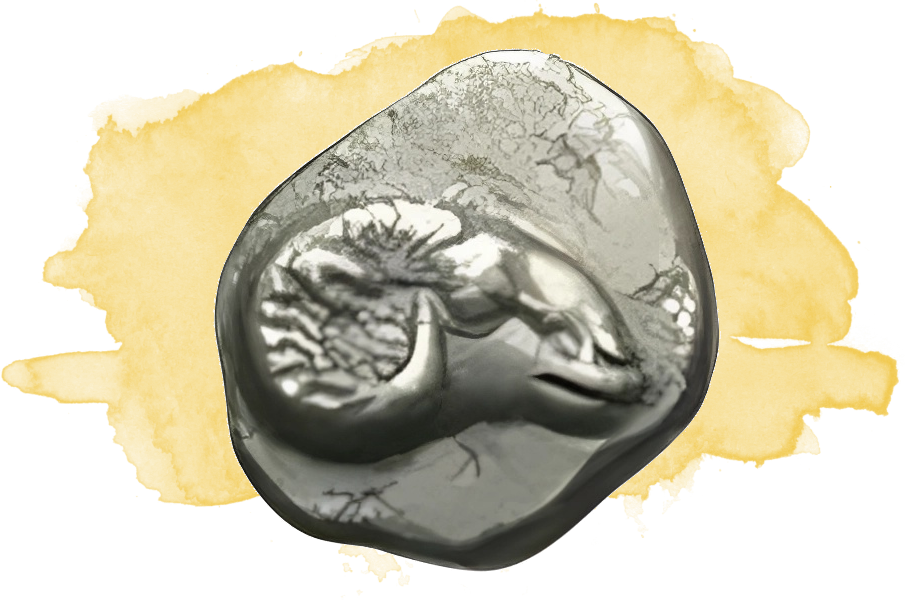
\includegraphics[width=0.9\columnwidth]{media/obolo-bhaal.png}
  \caption{El Óbolo de Bhaal}
\end{figure}

Esto le llevo a juntarse cada vez más con personas misteriosas y oscuras, y a realizar rituales
sobrenaturales. En una ocasión conoció a un cultista de Baal y este le entregó un objeto mágico
llamado óbolo de Bhaal que le podría cumplir el deseo de la juventud eterna. Con este objeto, 
Sirius contacto a Bhaal, el señor archidiablo de los nueve infiernos y del dominio de la muerte.
Bhaal, le sentencia que para cumplir su deseo, tendría que cometer un asesinato ritual una vez
cada decana en el momento más oscuro de la noche.

Aturdido por esto, Sirius quien nunca había tocado la sangre de nadie trata de deshacerse del 
Óbolo de Bhaal, primero lanzándolo desde su casa sin ver donde caía, luego llevándolo al bosque y 
cada vez más lejos. En todas las intentos de deshacerse el óbolo, al volver a casa, estaba ahí
siempre a la vista ante Sirius. Desesperado, intenta contactar a Bhaal con el óbolo nuevamente,
se corta la palma de la mano con un cuchillo, pero la herida desaparece al instante, se trata de
cortar la otra palma y ocurre lo mismo. Se pasa el cuchillo por la mejilla y la herida 
desaparece.

Evangeline va a visitar a Sirius ya que tenía días sin saber nada de él. Al llegar, una brisa 
gélida pero ominosa le acaricia el rostro. Se siente un poco aturdida, pero aún así decide entrar 
a Villa Argentum, en la sala de estar, donde estaba colgado el retrato de Lord Sirius que había 
hecho, lo examina detenidamente y ve una herida en la mejilla de Sirius que ella no había 
pintado. Se trepa en una silla para examinar la pintura de cerca y todo pareciera indicar que 
siempre estuvo ahí esa herida. En ese momento Sirius llega a la sala de estar y Evangeline le 
interroga sobre la pintura y Sirius le cuenta. Evangeline trata de quitarle el óbolo, al cual 
identifica como responsable de todo, pero Sirius se niega. Forcejean y sin darse cuenta que 
ocurrió, Lady Evangeline cae muerta frente a Sirius. Sirius tiene en sus manos el cuchillo que 
utilizo para hacerse las heridas, al ver a Evangeline tirada en el suelo, sus ropas comienzan a 
mancharse de sangre profusamente en el pecho.

Una voz como un susurro llega a sus oídos diciendo, “Bhaal te espera, Bhaal te abraza, nadie 
escapa a Bhaal”. En un intento desesperado por revivirla, trata de levantarla, despertarla. Solo 
hay silencio como respuesta y lo miran los ojos sin vida de Evangeline. Entonces decide ocultar 
el cuerpo y la pintura llevándola al subnivel del sótano y huye de la casa. 

Tres días después, angustiado regresa a su casa y decide volver al subnivel del sótano, el cuerpo 
de Evangeline yacía ahí, tal cual lo había dejado. No había ningún signo de putrefacción, ni olor 
nauseanbundo. Comprendió entonces que al no completar el ritual, el cuerpo de Evangeline seguiría 
intacto. Volvió a cortar su mano y la herida desapareció al instante. Entonces improviso una 
cripta removiendo los adoquines del suelo y cavando. Colocó la pintura en la pared más lejana a 
la entrada del sótano y decidió sellar el subnivel del sótano.

Como era cuestión de tiempo que la familia Vanthorn notara la ausencia de su hija, abandonó la 
casa y escondió el óbolo de Bhaal dentro de ella. Huyó. Tan lejos como pudo, se exilió. 

Aún atormentado por la muerte de Evangeline, refugiado en una oscura taberna en Luskan cerca
de medianoche, al salir fuera y subir las escaleras hacia las habitaciones. Un bandido de poca 
monta lo asalta e intenta asesinarle. Pero la herida se cerró al momento. Sirius sorprendido supo 
que el pacto con Bhaal se mantenía en vigencia. Ahí, en esa oscuridad, asesina a golpes al bandido.
Examinando las ropas del cadáver detenidamente reconoció en él un amuleto que colgaba del cuello
que identifica a los cultistas de Bhaal. Tomo el amuleto manchado de sangre y lee en voz alta 
la inscripción alrededor del amuleto. “Bhaal te espera, Bhaal te abraza, nadie escapa a Bhaal”.
Acto seguido, toda la sangre desaparece de sus manos y rostro y el cadáver se desvanece en jirones 
de polvo. Había consumado su primer asesinato en nombre de Bhaal.

\section{Villa Argentum}

La mansión Villa Argentum, fue construida por Lord Sirius Belmont I, hace unos cien años. Es una 
mansión amplia y ostentosa de 2 plantas, un sótano y un subnivel para las criptas familiares.
Con la muerte de Lady Evangeline Vanthorn, el nivel de las criptas fue sellado por Lord Sirius.
Al aproximarse a la mansión, las puertas se abrirán solas dejando pasar a los jugadores sin ningún 
problema. Una vez haya entrado el último, se cerrarán para no volver a abrirse.

Si los jugadores deciden investigar los alrededores de la casa, descubrirán que todas las ventanas
estan tapadas por tablones de madera. Y no se pueden romper de ninguna manera, como si algo 
mantuviera de forma artificial su integridad. Si se hace un conjuro de Detectar Magia, se verá que 
alrededor de toda la casa hay potentes auras mágicas de transmutación, abjuración y nigromancia. 

Una vez dentro, el contenido de la casa verán que está en perfecto estado. Alfombras, muebles, 
candelabros y lámparas estarán ilumninando en todo momento ardiendo como si no hubieran 
transcurrido 100 años.

\begin{figure}
  \centering
  \includegraphics[width=\columnwidth]{maps/villa-argentum-full1.png}
  \caption{Villa Argentum - Niveles PB y L1}
  \label{fig:vaf}
\end{figure}

\DndArea{Nivel PB}

\DndSubArea{Vestíbulo}

Luego que se cierren las puertas, los jugadores se encontrarán en el vestíbulo, con un escritorio 
al frente y sillas a la izquierda y derecha con una lujosa alfombra a sus pies. Una prueba de 
investigación les permitirá encontrar en las mesitas adyacentes a las sillas a los lados de la 
puerta algunas cartas que firma Evangeline.

Detrás del escritorio hay una pared que divide parcialmente el vestíbulo y de ella cuelga una 
enorme pintura de un paisaje y las lados dos lámparas con forma de cabeza de dragón doradas.
Verán también una gran cantidad de libros en los estantes alrededor del vestíbulo.

En la pared oeste del vestíbulo, entre las ventanas hay otra pintura colgada de unas frutas sobre 
un canasto. Una prueba de investigación sobre las pinturas permitirá deducir que al parecer ambas 
fueron hechas por la misma persona.

\DndSubArea{Sala de estar}

Al salir hacia la derecha del vestíbulo se encontrarán ante una sala de estar con dos sillas 
que miran hacia una pintura en la pared. En la pintura hay un paisaje montañoso que les parecerá
extrañamente familiar a los jugadores. Un jugador que haga una prueba de inteligencia con CD 12 
y la superé o que tenga un bonificador de historia le permitirá identificar el Pico Agujahelada.
También identificará que el autor sigue siendo el mismo.

\DndSubArea{Corredor}

En el pasillo verán dos pinturas más de paisaje, una prueba de investigación de una de ellas
les permitirá identificar una firma con iniciales EV y que probablemente es del mismo autor.
Escucharán también un sonido parecido al llanto de una mujer.

\DndSubArea{Biblioteca}

\DndSubArea{Baño de visitas}

\DndSubArea{Comedor}

\DndSubArea{Cocina}

\begin{figure*}[hb!]
  \centering
  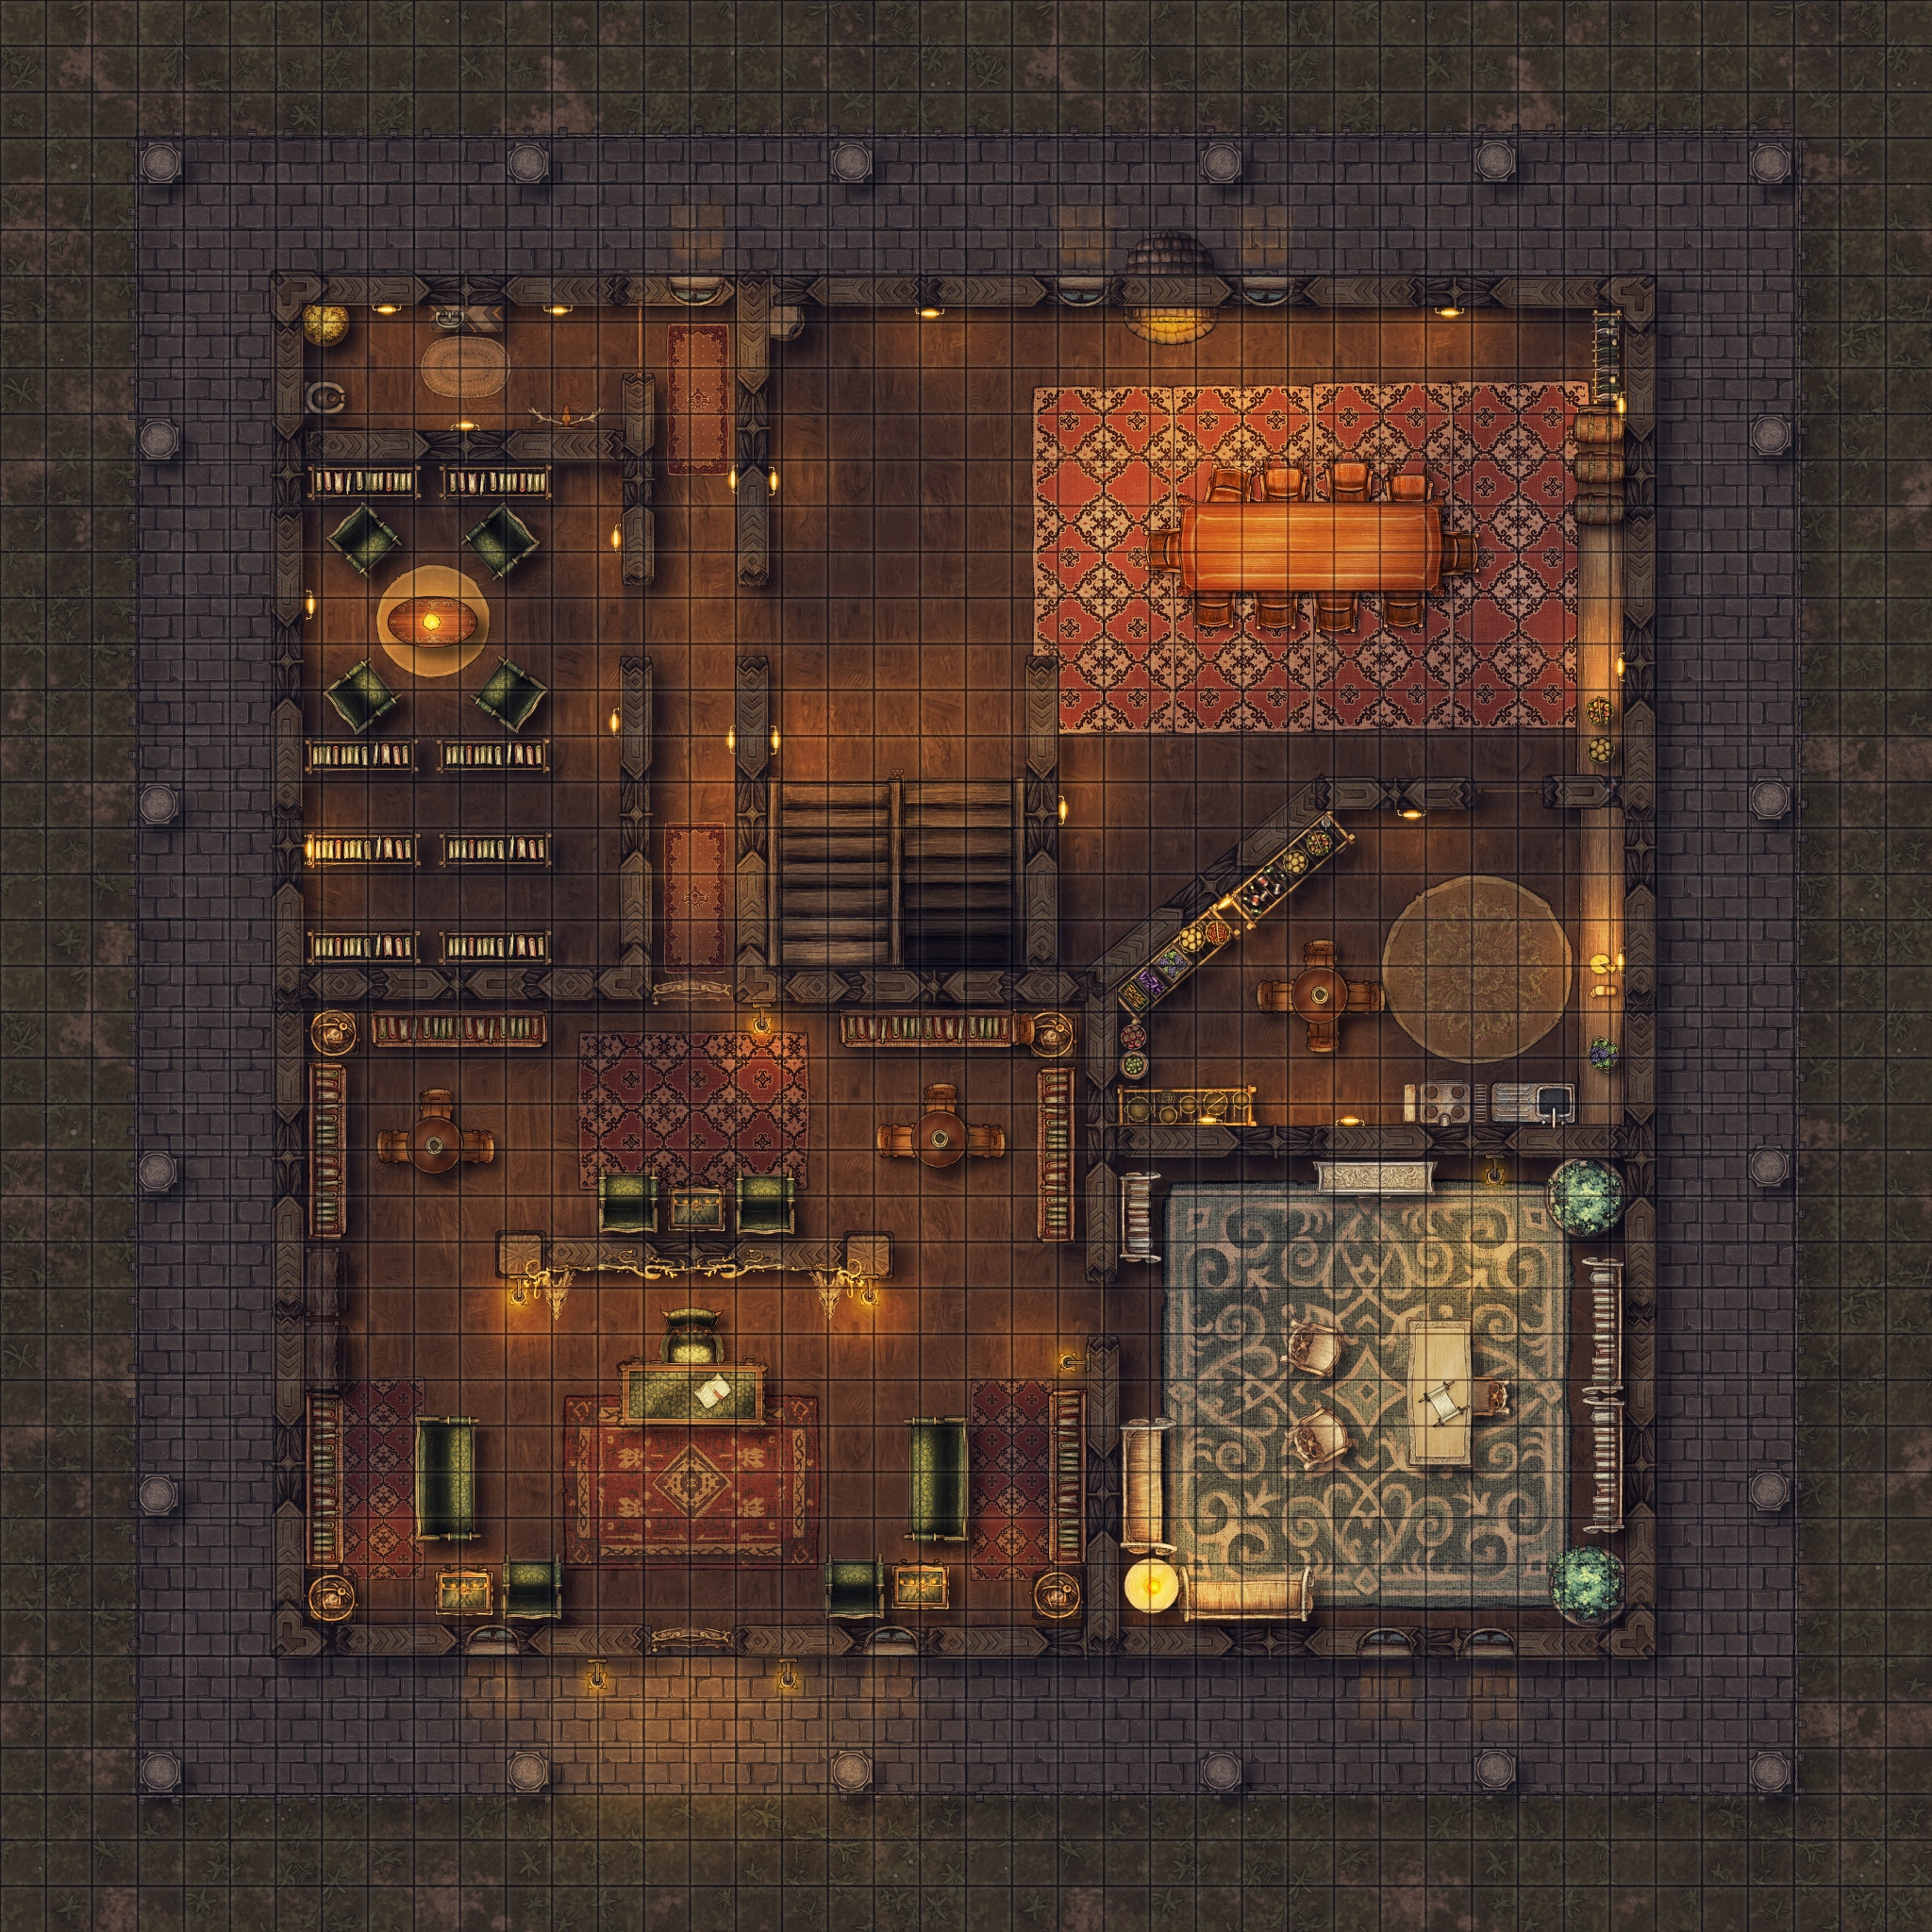
\includegraphics[width=\textwidth]{maps/villa-argentum-pb.jpg}
  \caption{Villa Argentum - Planta baja}
  \label{fig:vapb}
\end{figure*}



\begin{figure*}[hb!]
  \centering
  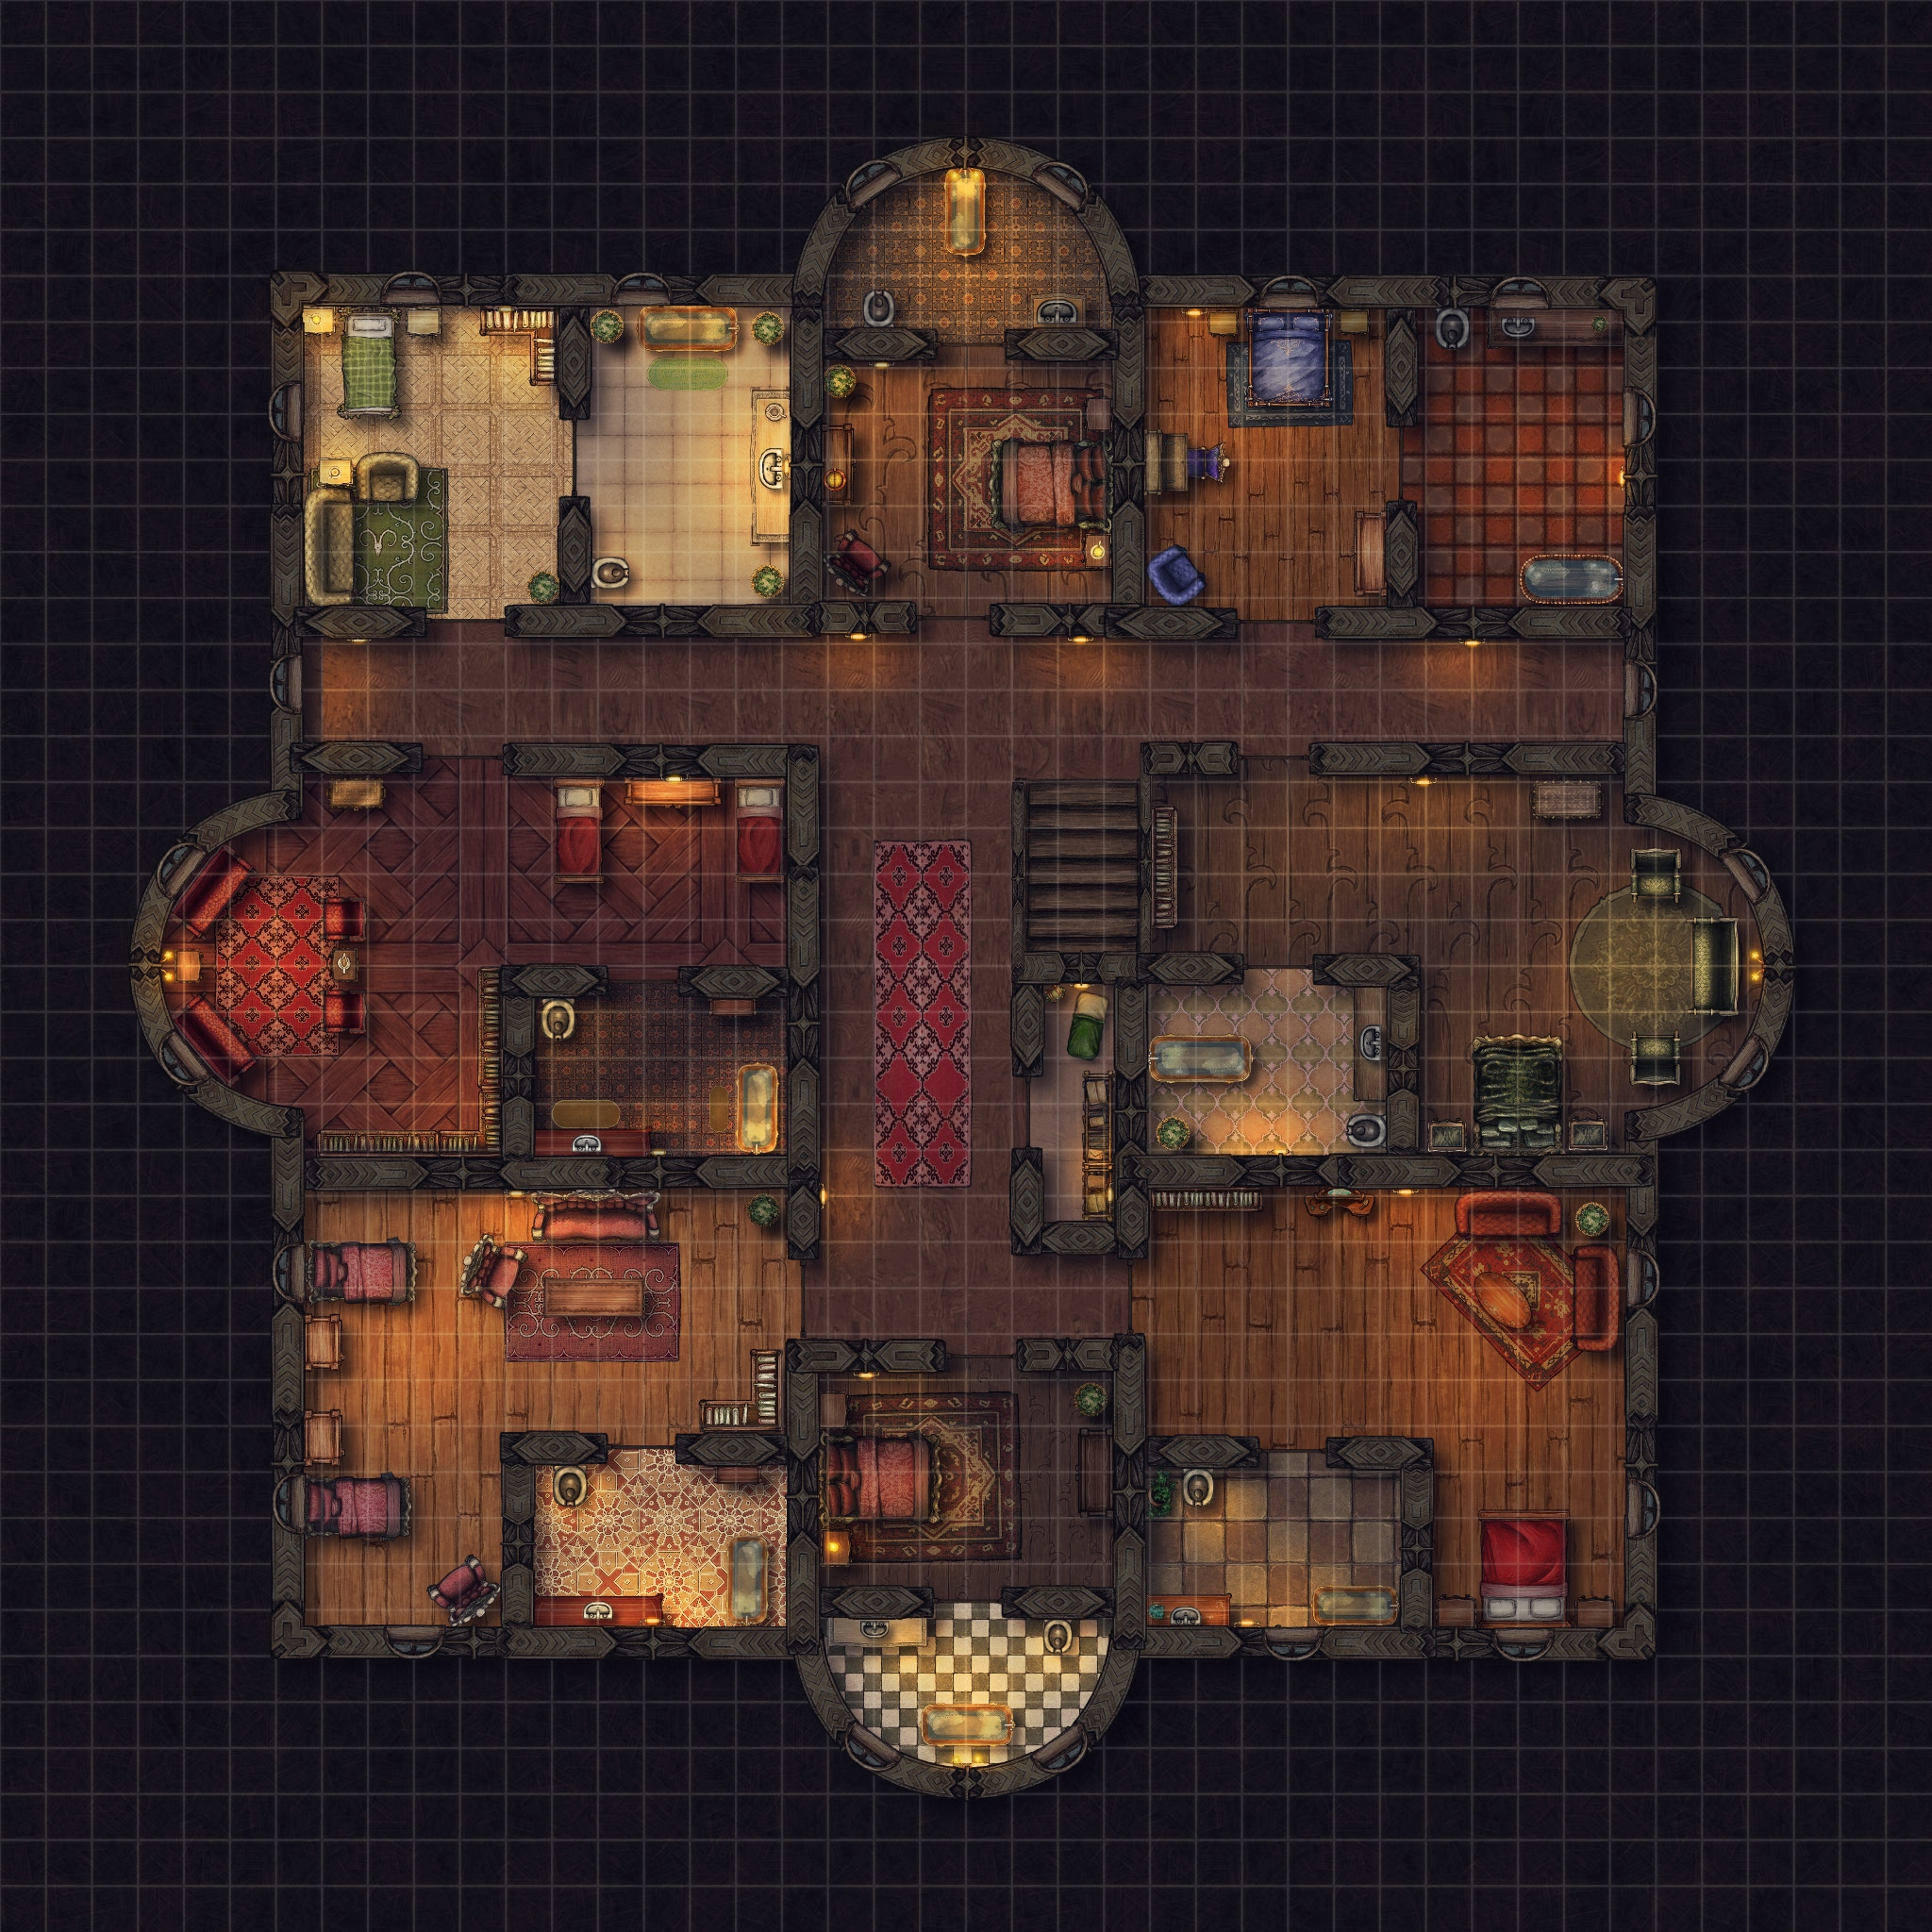
\includegraphics[width=\textwidth]{maps/villa-argentum-l1.jpg}
  \caption{Villa Argentum - Nivel superior}
  \label{fig:val1}
\end{figure*}

\begin{figure*}[hb!]
  \centering
  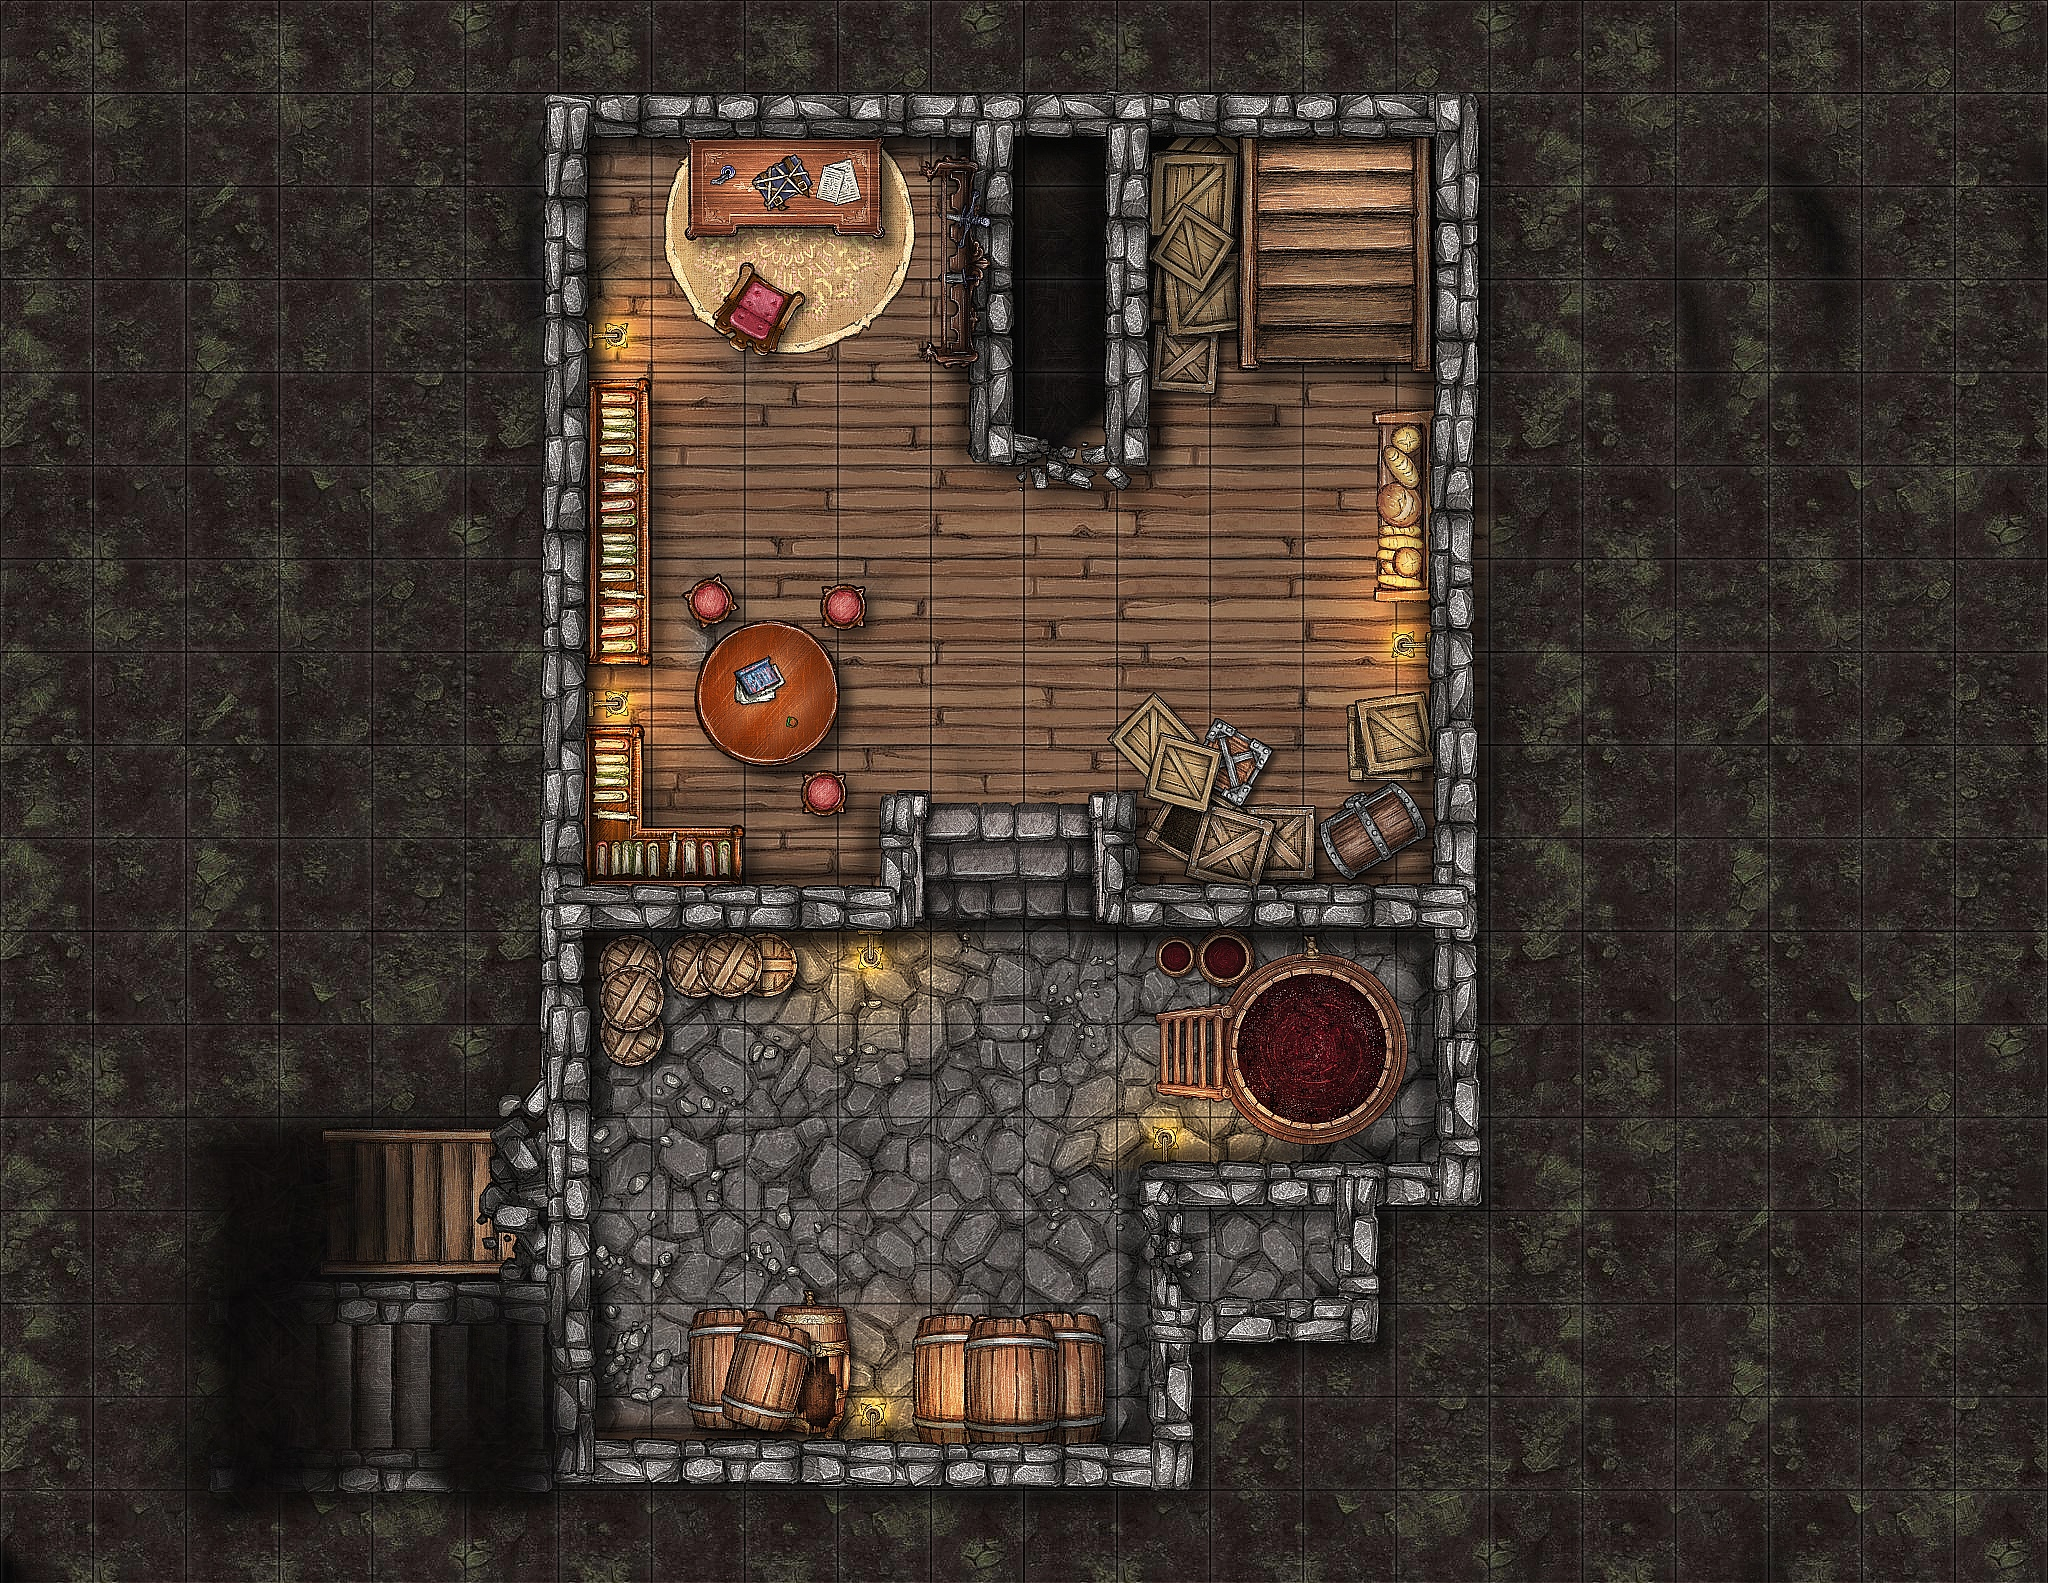
\includegraphics[width=\textwidth]{maps/villa-argentum-s1.jpg}
  \caption{Villa Argentum - Sótano}
  \label{fig:vas1}
\end{figure*}

\begin{figure*}[hb!]
  \centering
  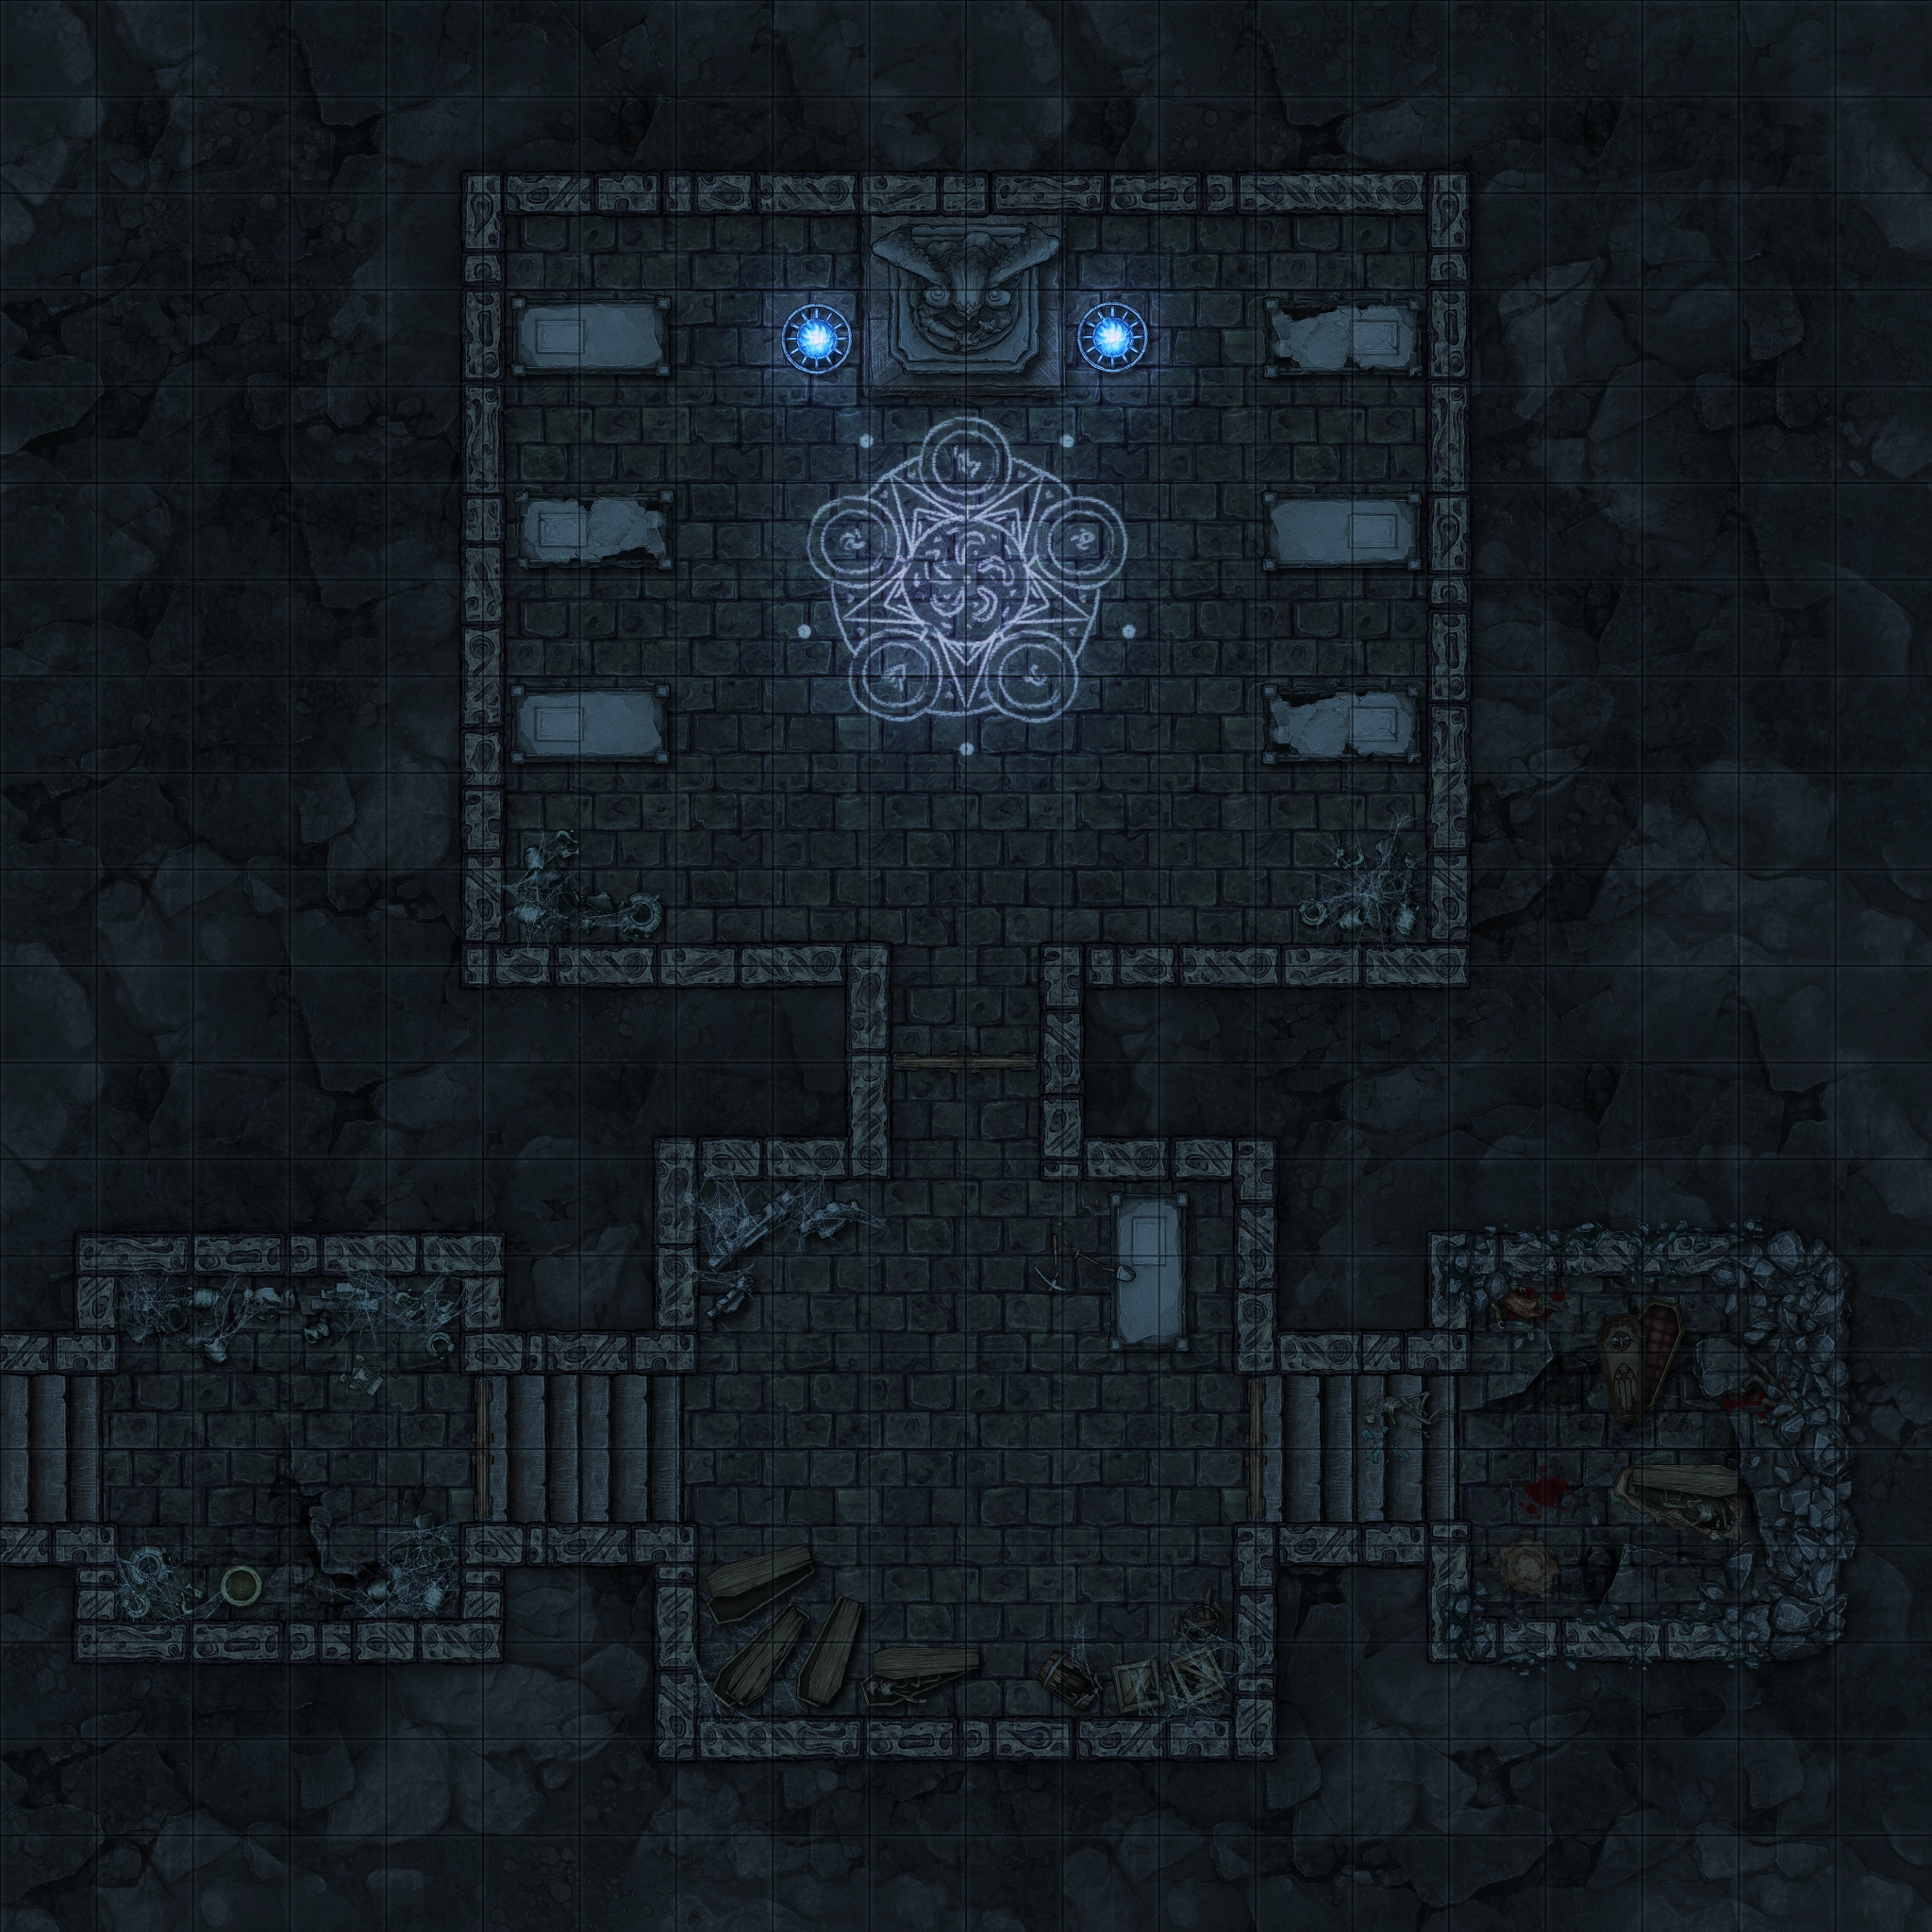
\includegraphics[width=\textwidth]{maps/villa-argentum-s2.jpg}
  \caption{Villa Argentum - Criptas}
  \label{fig:vas2}
\end{figure*}




\section{Créditos}

Las ilustraciones en este one shot, son creaciones de sus respectivos autores. Los mapas han sido 
creados con la herramienta \href{https://inkarnate.com/}{Inkarnate}. Las ilustraciones de los 
personajes no jugables, fueron creadas con la herramienta Leonardo.Ai. Estos son los enlaces a las 
ilustraciones originales:

\begin{itemize}
  \item Lord Sirius Belmont creada por \href{https://cdn.leonardo.ai/users/898407a5-5b36-4dae-87cc-c51a8041e826/generations/8ac651a0-9be3-4896-85f0-2ce0d8e01215/DreamShaper_v7_dungeon_and_dragons_style_illustration_charisma_1.jpg}{linkmoises en Leonardo.Ai}.
  \item Lady Elizabeth Vanthorn creada por \href{https://cdn.leonardo.ai/users/898407a5-5b36-4dae-87cc-c51a8041e826/generations/a5c78c2e-61f0-478a-8005-03b46068bcdc/DreamShaper_v7_dungeon_and_dragons_style_illustration_charisma_1.jpg}{linkmoises en Leonardo.Ai}.
  \item A day in Hell por \href{https://licensing.pixels.com/featured/a-day-in-hell-jackson-parrish.html}{Jackson Parrish}.
  \item Guild House L1 por \href{https://inkarnate.com/p/RVAA0X-criana/maps/79j1zW-guild-house/}{Criana en Inkarnate}.
  \item Guild House F2 por \href{https://inkarnate.com/p/RVAA0X-criana/maps/lZznw8-guild-house-f2/}{Criana en Inkarnate}.
  \item Basement and cave por \href{https://inkarnate.com/p/49vmYo-jared-fletcher/maps/kdGk9r-basement-and-cave/}{Jared Fletcher en Inkarnate}.
  \item Basement Ruins of an Old Library por \href{https://inkarnate.com/p/R1zAY7-rhasmus/maps/lJ1wxd-day-89-365-basement-ruins-of-an-old-library/}{Rhasmus en Inkarnate}.
\end{itemize}


\end{document}
